% This is samplepaper.tex, a sample chapter demonstrating the
% LLNCS macro package for Springer Computer Science proceedings;
% Version 2.20 of 2017/10/04
%
\documentclass[runningheads]{llncs}
\renewcommand{\baselinestretch}{1.1} 
%
\usepackage{graphicx}
\usepackage[table]{xcolor}
\usepackage{xspace}
\usepackage{hyperref}
\usepackage{subcaption}
\usepackage{listings}
\usepackage{ulem}

\usepackage[para,online,flushleft]{threeparttable}
\usepackage{booktabs}
\usepackage{multirow}
% \usepackage{geometry}
% \usepackage{marginnote}

% Fix link colors
\hypersetup{
    colorlinks = true,
    linkcolor=red,
    citecolor=red,
    urlcolor=blue,
    linktocpage % so that page numbers are clickable in toc
}

% Used for displaying a sample figure. If possible, figure files should
% be included in EPS format.
%
% If you use the hyperref package, please uncomment the following line
% to display URLs in blue roman font according to Springer's eBook style:
% \renewcommand\UrlFont{\color{blue}\rmfamily}
\newcommand{\TG}[1]{\noindent{\color{blue}[\textsc{From Tristan:} #1]}\xspace}
\newcommand{\Ali}[1]{\noindent{\color{green}[\textsc{From Ali:} #1]}\xspace}
\newcommand{\GK}[1]{\noindent{\color{purple}[\textsc{From Greg:} #1]}\xspace}
\newcommand{\YC}[1]{\noindent{\color{orange}[\textsc{From Yohan:} #1]}\xspace}
\newcommand{\anonymous}[1]{***\xspace}


\lstdefinestyle{customC}{
  belowcaptionskip=1\baselineskip,
  breaklines=true,
  xleftmargin=\parindent,
  language=C,
  showstringspaces=false,
  basicstyle=\scriptsize\ttfamily,
  keywordstyle=\bfseries\color[rgb]{0.580, 0.000, 0.827},
  %{purple!40!lightgray},
  commentstyle=\textit{\color{green!40!black}},
  identifierstyle=\bfseries\color{cyan!75!black},
  stringstyle=\color{orange},
  deletekeywords={double,float},
  classoffset=1, % starting new class
  otherkeywords={double,float},
  morekeywords={double,float},
  keywordstyle=\bfseries\color{green!55!black},
  classoffset=0
}

\begin{document}

\title{Comparing tool variability and numerical variability in fMRI analyses}

\author{Ali Salari$^1$, Co-authors$^2$, Tristan Glatard$^1$}

\authorrunning{Salari et al.}
% First names are abbreviated in the running head.
% If there are more than two authors, 'et al.' is used.

\institute{$^1$ Anonymous Organization1\\
  $^2$ Anonymous Organization2\\ **@******.***}

\institute{$^1$ Department of Computer Science and Software Engineering, Concordia University\\
  $^2$ Co-authors Organization\\  Montréal, QC, Canada}

\maketitle              % typeset the header of the contribution

\begin{abstract}
abstract\dots

%  \keywords{Computational reproducibility  \and Neuroimaging pipelines \and Monte-Carlo arithmetic.}
\end{abstract}


\section{Introduction}

\begin{description}
  \item[$\bullet$ ] Methodological choice can influence the final determining areas of brain activation. This opens so results flexibility~\cite{bowring2019exploring}. 

  \item[$\bullet$ ] We presented a framework that can investigate the numerical instability of the pipelines based on Monte-Carlo arithmetic
                    by creating a Fuzzy environment, so that instrument mathematical functions implemented in mathematical system libraries (libmath). 

  \item[$\bullet$ ] In this paper, we aim to answer the questions 1) how the fMRI analyses are numerically stable?
                    2) how the numerical variability is in comparison with the tool variability?
\end{description} 


\section{Methodology}

\subsection{Fuzzy libmath environment}

% To simulate the machine level uncertainty, we used the method introduced in~\cite{FL-MICAII-paper} called Fuzzy libmath (FL).
% FL uses Monte Carlo Arithmetic (MCA) to introduce a controlled amounts of noise in the floating-point operations,
% which models floating-point rounding and catasrophic cancellation errors.
% This is automated using Verificarlo tool~\cite{denis2015verificarlo} that implements MCA in the compilation time.
% The perturbation is introduced in a given number of least-significant bits so that
% the number of bits in the mantissa that will not be perturbed is defined as the virtual precision.​

% % MCA models floating-point roundoff and cancellations errors through random
% % perturbations, allowing for the estimation of error distributions from
% % independent random result samples. MCA simulates computations at a given
% % \emph{virtual precision} using the following perturbation:
% % \begin{equation} \label{eq:mca_inexact}
% %   inexact(x) = x + 2^{e_x-t}\xi
% %   \label{mcadefinition}
% % \end{equation}
% % where $e_x$ is the exponent in the floating-point representation of $x$,
% % $t$ is the virtual precision and $\xi$ is a random uniform variable of
% % $(-\frac{1}{2}, \frac{1}{2})$.

% % MCA allows for three perturbation modes: Random Rounding (RR) introduces the
% % perturbation in function outputs, simulating roundoff errors; Precision Bounding
% % (PB) introduces the perturbation in function operands, allowing for the
% % detection of catastrophic cancellations; and, Full MCA combines RR and PB,
% % resulting in the following perturbation:
% % \begin{equation} \label{eq:mca_modes}
% %   mca\_mode(x \circ y) = inexact_{RR}(  inexact_{PB}(x) \circ inexact_{PB}(y) )
% % \end{equation}

% % We instrumented the GNU mathematical library with MCA using
% % Verificarlo~\cite{denis2015verificarlo}, a tool that (1) uses the Clang
% % compiler to generate an LLVM (\url{http://llvm.org}) Intermediate
% % Representation (IR) of the source code, (2) replaces floating-point operations
% % in the IR by a call to the Verificarlo API, and (3) compiles the modified IR to
% % an executable using LLVM. The perturbation applied by the Verificarlo API
% % can be configured at runtime, for instance to change the virtual
% % precision applied to single- and double-precision floating-point values.

% In this framework, mathematical functions embeded in the operating system GNU mathematical library (libmath)
% are targeted to be instrumented.
% It instrument the functions by wrapping them so that only the output of the original functions be perturbed
% instead of input or their implementation.
% This is achieved by adding a floating-point zero to the output of the original function which results into perturbations.
% Script~\ref{script1} shows an example of this wrapping for the log function.
% This functionality helps to avoid of some issues in deterministic arithmetics like producing results out of the function definition.


% % To simulate OS updates, we introduce random perturbations in the GNU
% % mathematical library, the main mathematical library in GNU/Linux systems.
% % Instrumenting mathematical libraries with MCA raises a number of issues as
% % many functions assume deterministic arithmetic. For instance, applying random
% % perturbations around a discontinuity or within piecewise approximations
% % results in large variations and a total loss of significance that are not
% % relevant in our context. Therefore, we have applied MCA to proxy
% % mathematical functions wrapping those in the original library, such that only
% % the outputs of the original functions were perturbed but not their inputs or
% % the implementations themselves. This technique allows us to control the
% % magnitude of the perturbation as perceived by the application.

% \lstset{
%   language=C,                % choose the language of the code
%   numbers=left,                   % where to put the line-numbers
%   stepnumber=1,                   % the step between two line-numbers.        
%   numbersep=5pt,                  % how far the line-numbers are from the code
%   backgroundcolor=\color{white},  % choose the background color. You must add \usepackage{color}
%   showspaces=false,               % show spaces adding particular underscores
%   showstringspaces=false,         % underline spaces within strings
%   showtabs=false,                 % show tabs within strings adding particular underscores
%   tabsize=2,                      % sets default tabsize to 2 spaces
%   captionpos=b,                   % sets the caption-position to bottom
%   breaklines=true,                % sets automatic line breaking
%   breakatwhitespace=true,         % sets if automatic breaks should only happen at whitespace
% %  title=\lstname,                 % show the filename of files included with \lstinputlisting;
% }
% \lstinputlisting{wrapper.c}
% %\lstinputlisting{wrapper2.c}

% The instrumented math functions so called ``fuzzy libmath", is loaded in the pipeline using LD\_PRELOAD, a Linux mechanism
% to force load a shared library into an executable. ​
% As a result, functions defined in fuzzy libmath transparently overload the original ones without the need to modify or
% recompile the analysis pipeline.​
% Also, this technique allows measuring the effect of numerical noise by running a program multiple times.​
% It is important to review the software dependencies of the pipelines to be sure that are involved with the same library that
% we arep erturbing.

% % The resulting MCA-instrumented mathematical library, ``fuzzy libmath" (FL), is
% % loaded in the pipeline using \texttt{LD\_PRELOAD}, a Linux mechanism to
% % force-load a shared library into an executable. As a result, functions defined in fuzzy libmath
% % transparently overload the original ones without the need to modify
% % or recompile the analysis pipeline. Fuzzy libmath functions call the original
% % functions through \texttt{dlsym}, a function that returns the memory address of
% % a symbol. To trigger MCA instrumentation, a floating-point zero is added to the
% % output of the original function and the result of this sum is perturbed and
% % returned.

% % \begin{description}
% %   \item[$\bullet$ ] libmath Fuzzy allows you to study the numerical stability of tools and pipelines. 
% %   \item[$\bullet$ ] It is based on MCA perturbations so that applies slight noise on floating-point operations.
% %   \item[$\bullet$ ] It does not need source code modification or recompilation, and simply works using the Linux LD\_PRELOAD environment variable.
% %   \item[$\bullet$ ] The library call interposition technique enables us to assess the tools that are dynamically linked to the mathematical library.
% % \end{description} 


\subsection{fMRI analyses \& Dataset}

% We replicate the fMRI analysis (ds000001 study) used in~\cite{bowring2019exploring} with the publicly available
% data repository in~\href{https://openneuro.org/datasets/ds000001}{OpenNeuro}
% using the three most popular packages for fMRI data processing including FSL, AFNI, and SPM. 
% We selected this publication to replicate the fMRI analysis because it is an state of the art study
% which compares between tool variability, and included all the sources and dataset available
% so that we can easility reanalyse tests using Fuzzy framework.
% A full description of the procedure of analysis is included in~\cite{bowring2019exploring,schonberg2012decreasing};
% we give a brief overview of the pipeline processes in this section.
% In this study, 16 healthy adult subjects participated in the balloon analogue risk task to measure risk-taking behavior
% over three scanning sessions.
% %The analysis was scripted using three different tools so that 
% In the original study, a number of preprocessing steps which are widely accepted within the community
% such as motion correction, segmentation, brain extraction, and registration 
% were applied in all of the analyses to ensure that results from each software package could be compared objectively.
% % The steps that are taken in the procedure of analysis for each tool is specified in table~\ref{table:fmri-steps}.
% The analysis includes preprocessing, first-level, and second-level steps (Table~\ref{table:fmri-steps}) in all three software\dots


\subsection{Data processing}

% The fMRI analysis pipeline was processed using three of the most popular software packages in neuroimaging
% including FSL (version 5.0.10), AFNI (version 18.1.09), and SPM (version SPM12, r7771) on Octave (version 5.2).
% The analyses were conducted on the same operating system, CentOS 7.3.
% We ensured that the software versions and all the requisites for running analyses used in all experiments 
% are similar to the original study, and were encapsulated in Docker images.
% We could replicate results of the original study except for AFNI with slightly differences due to the parallelization\dots
% We also used SPM/Octave instead of Matlab to be able to run analysis in HPC and also perturb mathmetical functions
% because Matlab has no dependencies on the GNU mathematical library, and it uses its libraries\dots

% In addition, we processed the same pipeline analyses with the same configurations in Fuzzy libmath environment
% to capture the numerical variability results. 
% We only perturbed the maximum precisions to compare uncertainty between tool variability and numerical instability at the level of OS.
% For this purpose, we instrumented to the virtual precision (t) of 53 bits for double-precision variable,
% and 24 bits for single-precision variable. We generated three Fuzzy samples in these precisions to match the number of tool samples.

% We compare variability between (un)thresholded of group-level activation maps.
% We statistically compute standard deviations between T-statistic values in the pair of tools.
% We calculate standard deviations between fuzzy samples as the square root of summation of variances between Fuzzy samples in each tool.
% We then compare the correlation of changes in both conditions.
% Moreover, we compute region-by-region Dice coefficients for the thresholded maps for the all pairs of tools.
% This measures the overlap of voxels which assess the spatial similarity between activated maps.
% The Dice values between Fuzzy samples correspond to the average of Dices computed among three Fuzzy samples for each pair of tools.
% We then compare the correlation of Dice scores which normalized by the region sizes in both conditions.

% % EC is a means to assess whether only superficial scaling differences (differences by a scale factor over all voxels) 
% % are responsible for disparities between pair of images.


\section{Results}

All scripts and results to create the figures in this section are available on GitHub repository
in \url{https://github.com/ali4006/fuzzy-neurotools}.
Replication of all analyses was visually assessed to be the same as the original findings.
We ensured that fMRI analyses were processed successfully.
In this section, we call the cross-software variation and numerical variation,
between tool (BT) and within tool (WT) variability, respectively. 
The within tool variability shows results among different fuzzy libmath
samples for the specific version of the tools, and it is not within tool versions.


A summary of the statistic values from the group-level (un)thresholded T-statistics is conducted in
Table~\ref{table:pipeline-stats}.
The variability between pair of images in each condition was measured using the mean and standard deviation of absolute differences.
% Overally, we see that values in between tools are comparable to values in within tool results.
% The distribution of the pairwise differences in T-statistic..
% The standard deviations exceeding 2.0 in magnitude..
% Pairwise correlations ranged from 0.43 to 0.7 for within tool variability..


%%%%%%%%%% Summary of statstics %%%%%%%%
\setlength{\tabcolsep}{10pt}
\begin{table}[h]
    \centering
    \begin{tabular}{ccc|cc}
        \toprule
        \multirow{2}{*}{} & \multicolumn{2}{c}{Thresholded} & \multicolumn{2}{c}{Unthresholded} \\
        \cmidrule{2-3} \cmidrule{4-5} \\
        {} & Mean diff. & Std. diff. & Mean diff. & Std. diff. \\
        \midrule
        \rowcolor{lightgray}
        FSL vs. SPM          &  0.043       & 1.282      & 0.242     & 0.443  \\
        \rowcolor{lightgray}
        FSL vs. AFNI         &  0.099       & 1.548      & 0.302     & 0.547  \\
        \rowcolor{lightgray}
        AFNI vs. SPM         &  0.079       & 1.475      & 0.254     & 0.608  \\
        Fuzzy FSL and SPM    &  0.005       & 0.358      & 0.030     & 0.099  \\
        Fuzzy FSL and AFNI   &  0.011       & 0.475      & 0.038     & 0.155  \\
        Fuzzy AFNI and SPM   &  0.011       & 0.458      & 0.033     & 0.144  \\
        \bottomrule
    \end{tabular}
    \caption{Summary of T-statistics mean and standard deviation of differences for each pair of tools.}
    \label{table:pipeline-stats}
\end{table}


% \subsection{Comparing disparity in BT and WT}
\subsection{Spatial localization of disparity in BT and WT}
% Fig message: showing the magnitude of differences and correlated area
% Fig message: showing numerically dependent parts of the brain

%Fig 1,3
Comparisons of standard deviations between results in WT and BT
on the brain surface are shown in Figure~\ref{fig:thresh-varmaps} and Figure~\ref{fig:unthresh-varmaps}.
Figure~\ref{fig:thresh-varmaps} shows maps for group-level thresholded T-statistics, and
Figure~\ref{fig:unthresh-varmaps} shows maps for group-level unthresholded T-statistic values.
While we observe substantial variations in BT (average std. dev. $\approx$ 1.5),
the order of magnitude of variations in WT is much lower (average std. dev. $\approx$ 0.5),
as was anticipated. However, numerical variability is still significant in WT results.
Moreover, we see the same order of magnitude in WT variations compared to BT variations
in some regions in the thresholded images.
For instance, we see the temporal lobe in anterior view for almost all pairs and the fusiform gyrus in inferior view
for the pairs of FSL-SPM and FSL-AFNI in Figure~\ref{fig:unthresh-varmaps}
that are perfectly replicated using the numerical perturbations. 
Although the unthresholded statistic maps from our analyses also show a different magnitude of
the order of variations in both conditions, std. dev. ranges from $\approx$ 0.12 to $\approx$ 0.5 on average in WT and BT;
there is great comparability between results.
Generally, we obtained more uncertainty on thresholded results, probably due to different thresholding
methods used in different tools.
This can raise further investigations on the thresholding techniques toward stability.

% Fig2
In Figure~\ref{fig:dice-thresh}, we compare region-by-region Dice coefficients of
the group level thresholded maps in BT and WT for all pairs of software packages.
Results show that the similarity between tool variations is correlated with the numerical variations,
which implies that similar anatomical regions are activated, and also the topology of the activation patterns
is preserved between results from two types of variations.
% This correlation highly increases when normalizing Dice scores by the region sizes.
% which reduces the effect of small regions.

% This implies that region by region similarity between two type of variations are preserved.
% Results show that similar anatomical regions are activated in both conditions. 
% This plot suggests the similar topologies of the activation patterns in each condition.
% The average of Dice scores range from to 
% FSL-AFNI variations has the most similarity correlations which means that the results of these two tools are more \dots

% In response to the out of border activated voxels can say:
% This is likely due to the fact that SPM consistently had the smallest analysis mask out of the three packages,
% while FSL had the largest. Number of activated voxels prove this fact.

% Fig4
The scatter plot in Figure~\ref{fig:correlations} represents the correlation of standard deviation between conditions.
We found three major clusters, including upper, lower, and identity.
The identity cluster corresponds to the correlations between 0.9 and 1.1; the upper cluster shows correlations where BT $\approx$ 0;
and the lower cluster represents correlations where WT $\approx$ 0.
The identity area is also represented on the surface maps in the second row in Figure~\ref{fig:correlations}.
This figure shows the spatial localization of the parts of the brain that are numerically dependent.
We can see regions such as the occipital lobe in the posterior view and the frontal lobe in the interior view 
that are highly correlated in BT and WT results.
This refines the presented results in Figure~\ref{fig:unthresh-varmaps},
which indicates how spatial variabilities are simulated using numerical perturbations in some areas.
% Spatial localization of significant activation in the thresholded images also varied across software packages.
% Moreover, results show that pair of FSL-SPM has the least correlation of variability in within tool and between tool.
% This will implies that ... which can help for further investigations. 

% Mentioning P-values as well.
% Percentage of voxels in each cluster of Fig4
% fsl-spm
% Fraction of green: %9.9
% Fraction of purple: %0.7

% fsl-afni
% Fraction of green: %17.5
% Fraction of purple: %0.6

% afni-spm
% Fraction of green: %13.9
% Fraction of purple: %0.5



%%%%%%%%%% Var. of Thresh %%%%%%%%
\begin{figure}[ht]
  \fbox{\begin{minipage}{\dimexpr \textwidth-2\fboxsep-2\fboxrule}
  \begin{subfigure}[t]{\linewidth}
    \centering
    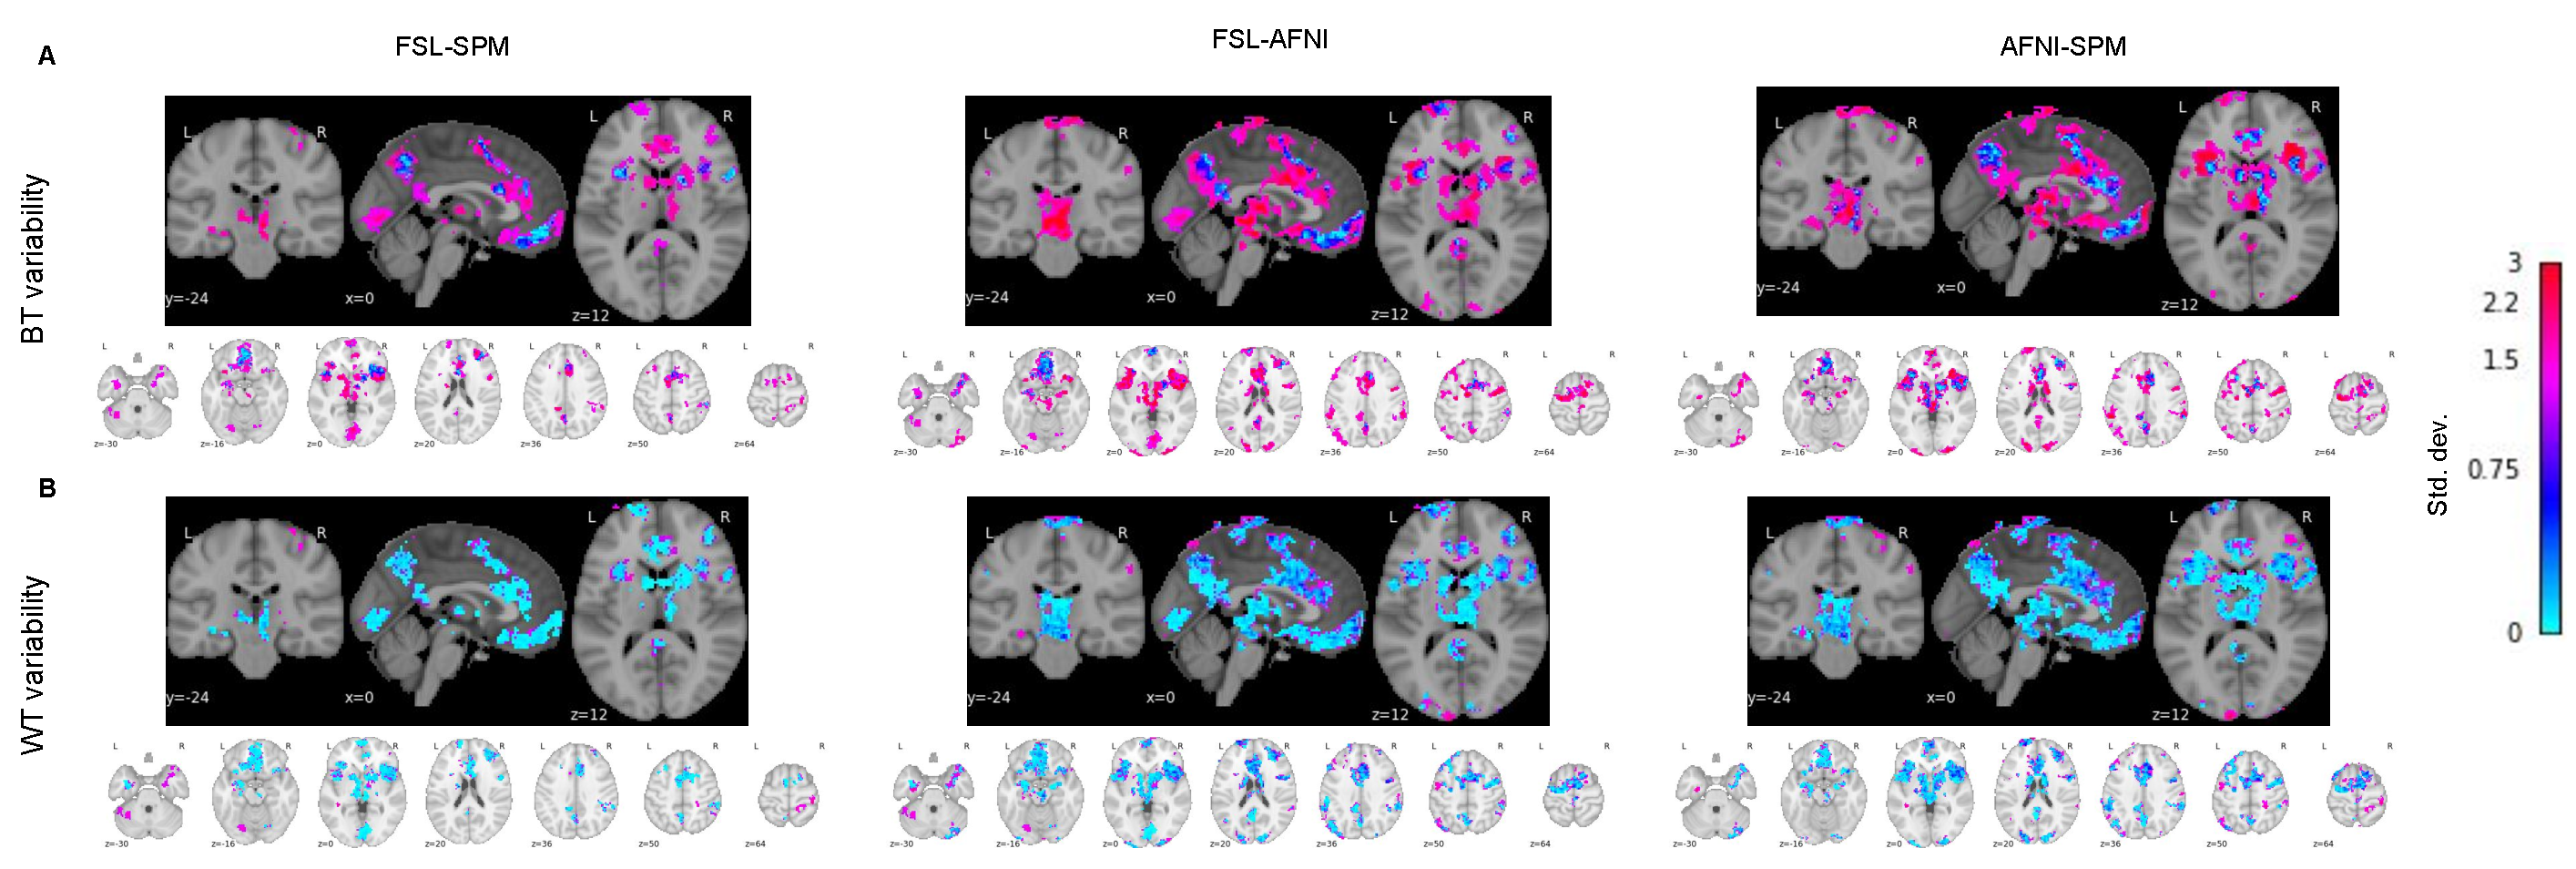
\includegraphics[width=\linewidth]{figures/plots/bt-wt-thresh-std.pdf}
    %\caption{Standard deviation of thresholded t-statistics map on template surface}
    \label{fig:thresh-varmaps1}
  \end{subfigure}
  \hfill
  \begin{subfigure}[t]{\linewidth}
    \centering
    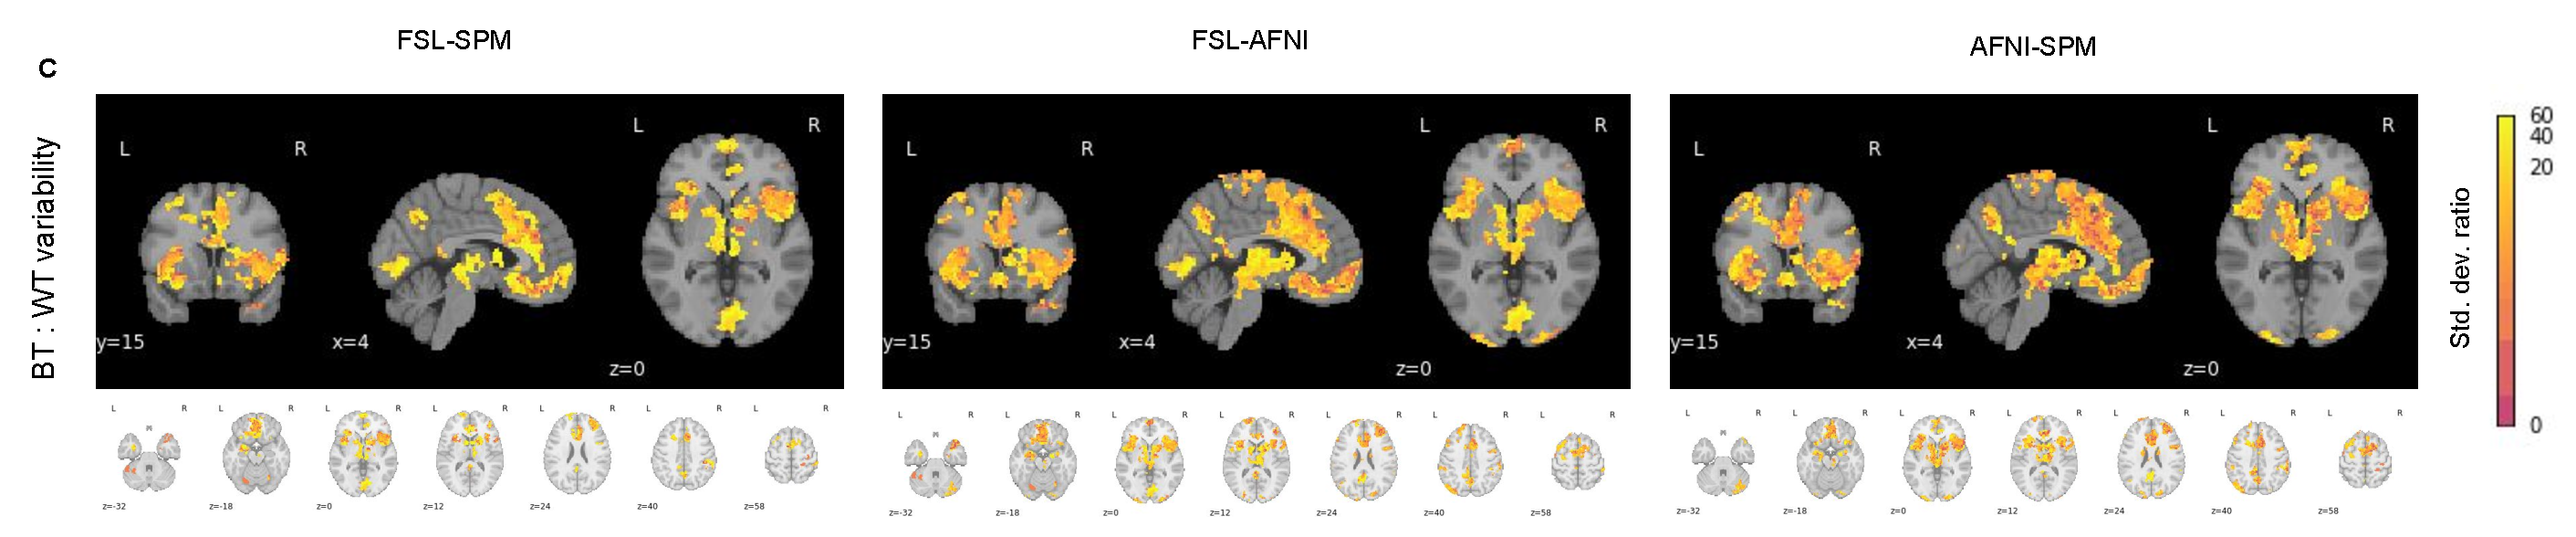
\includegraphics[width=\linewidth]{figures/plots/ratio-thresh-std.pdf}
    %\caption{Standard deviation of thresholded t-statistics map on template surface}
    \label{fig:thresh-ratiomaps}
  \end{subfigure}
  \caption{Maps of standard deviation of thresholded T-statistics. First and second rows show
  maps on between-tool and within-tool results, respectively. Third row represents the ratio of differences
  in between and within tools.}
  % so that bright blue areas indicate more similar order of magnitude of variations in both conditions,
  %and vise versa for the darkder regions.}
  \label{fig:thresh-varmaps}
  \end{minipage}}
\end{figure}


%%%%%%%%%% Dice plot of thresholded tstats%%%%%%%%
\begin{figure}[b]
  \fbox{\begin{minipage}{\dimexpr \textwidth-2\fboxsep-2\fboxrule}
  \centering
  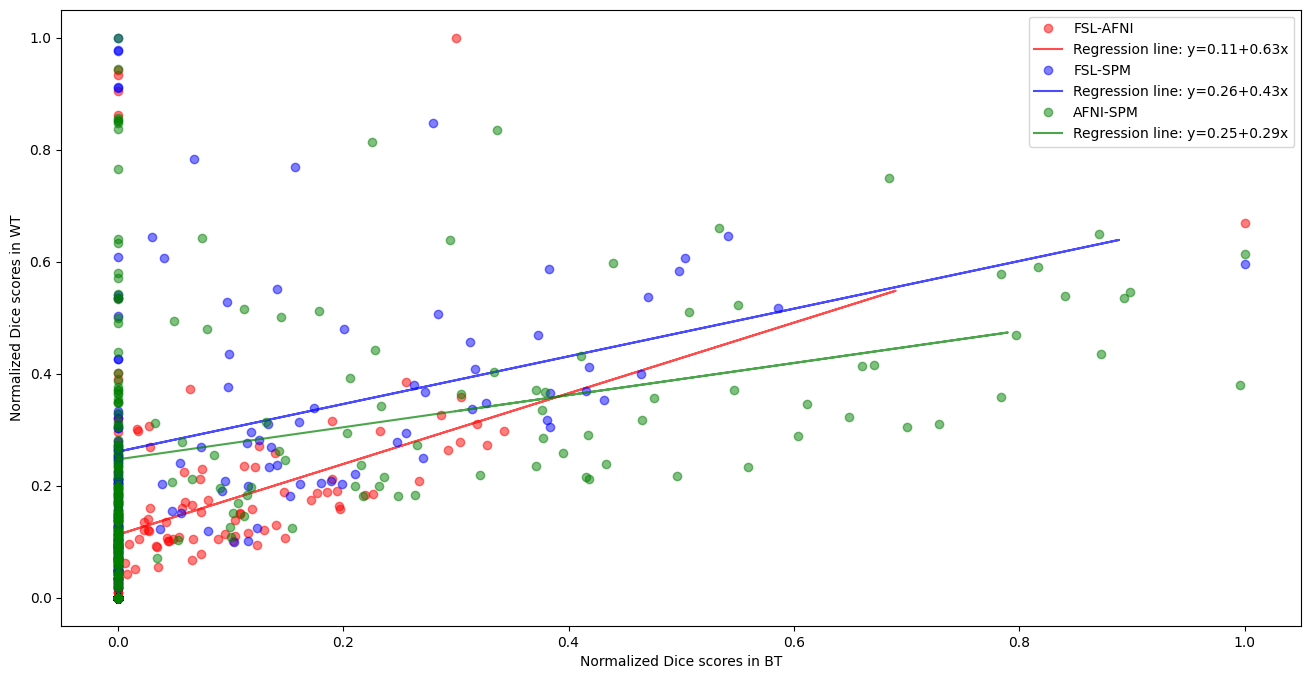
\includegraphics[width=\textwidth]{figures/dices_corr.png}
  \caption{Correlation of Dice coefficients of activated regions between pair of tools and fuzzy samples
  from the thresholded T-statistics. Different pairs are illustrated in different colors. 
  Regions correspond to the 360 areas of cortical parcellation (HCP-MMP1.0)~\cite{Glasser-nature}.}
  \label{fig:dice-thresh}
\end{minipage}}
\end{figure}



%%%%%%%%%% Var. of Thresh %%%%%%%%
\begin{figure}[b]
  \fbox{\begin{minipage}{\dimexpr \textwidth-2\fboxsep-2\fboxrule}
  \begin{subfigure}[t]{\linewidth}
    \centering
    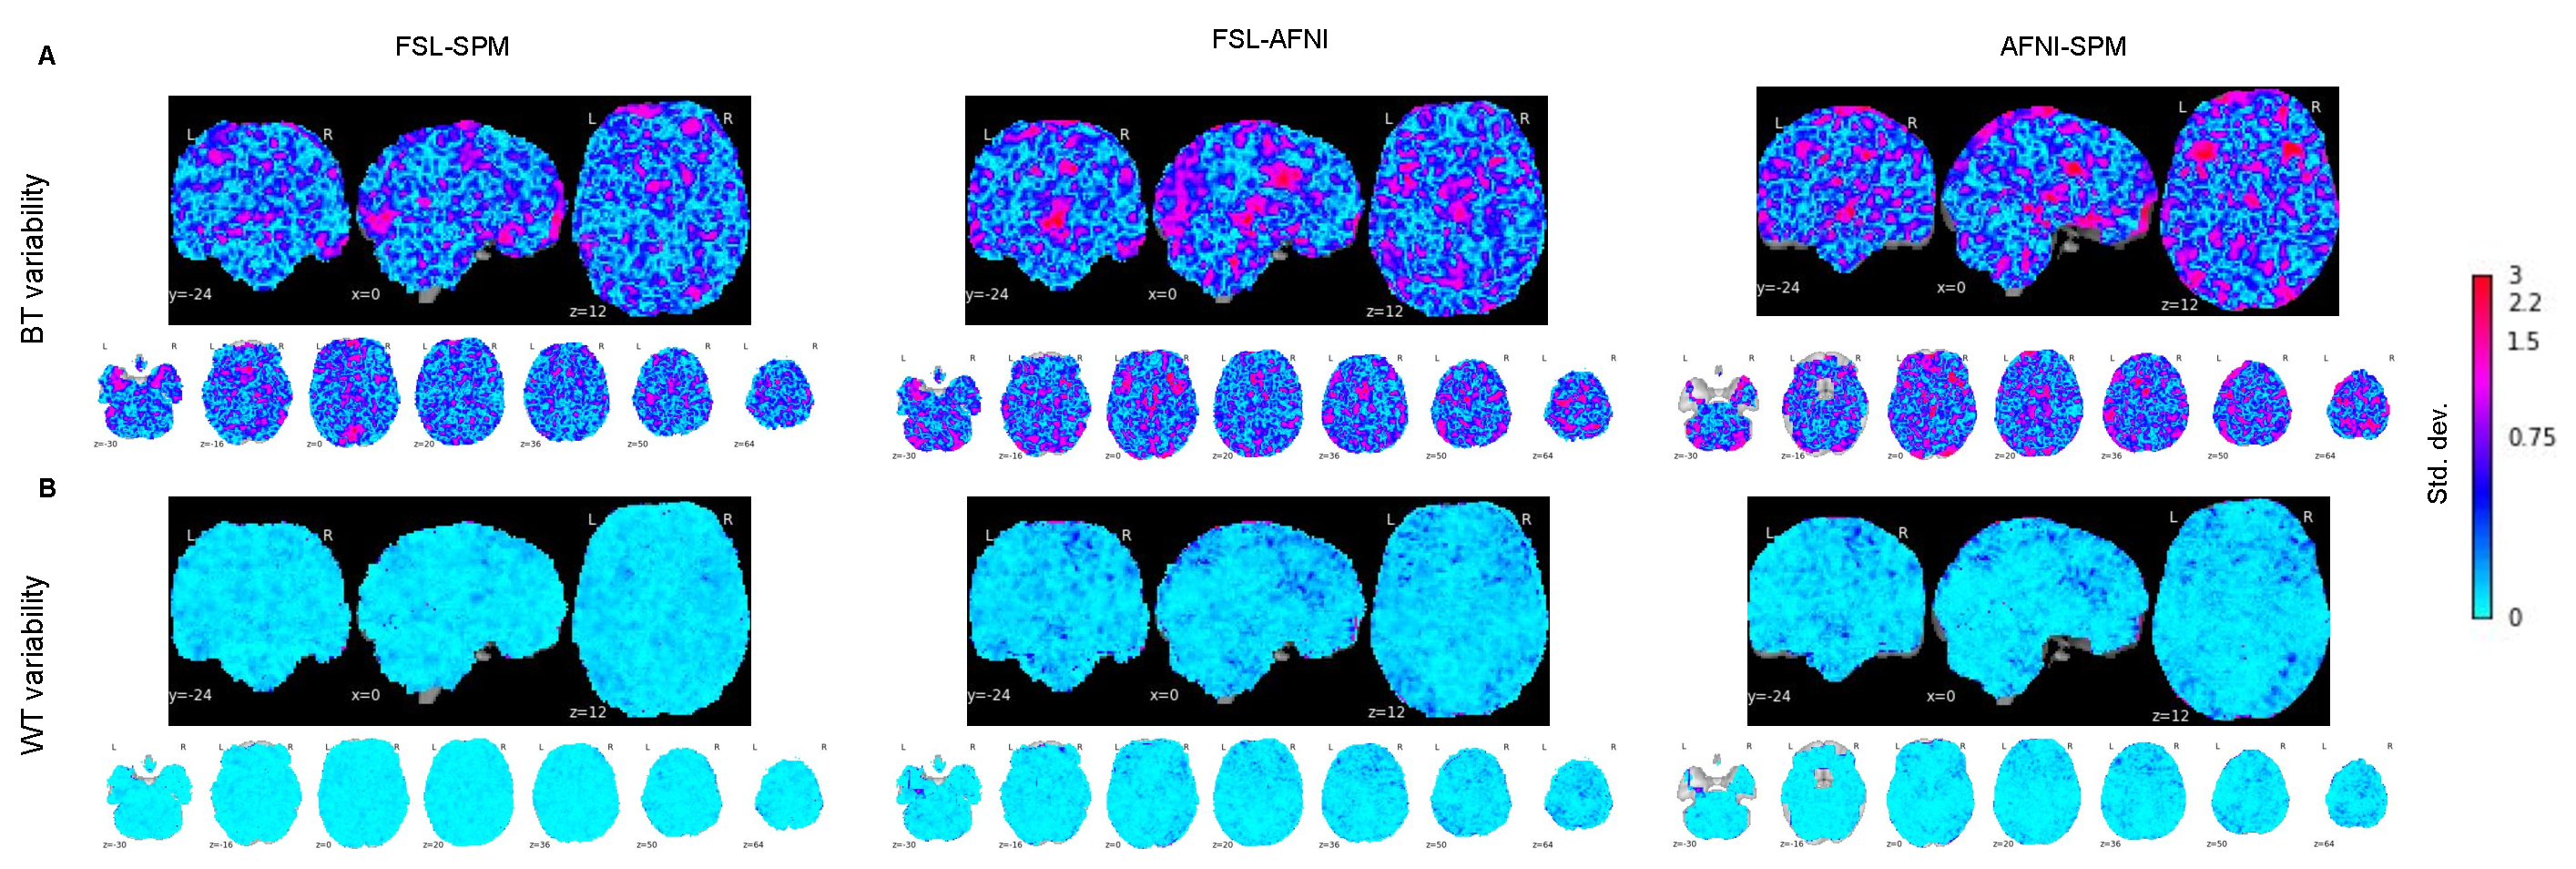
\includegraphics[width=\linewidth]{figures/plots/bt-wt-unthresh-std.pdf}
    %\caption{Standard deviation of thresholded t-statistics map on template surface}
    \label{fig:unthresh-varmaps1}
  \end{subfigure}
  \hfill
  \begin{subfigure}[t]{\linewidth}
    \centering
    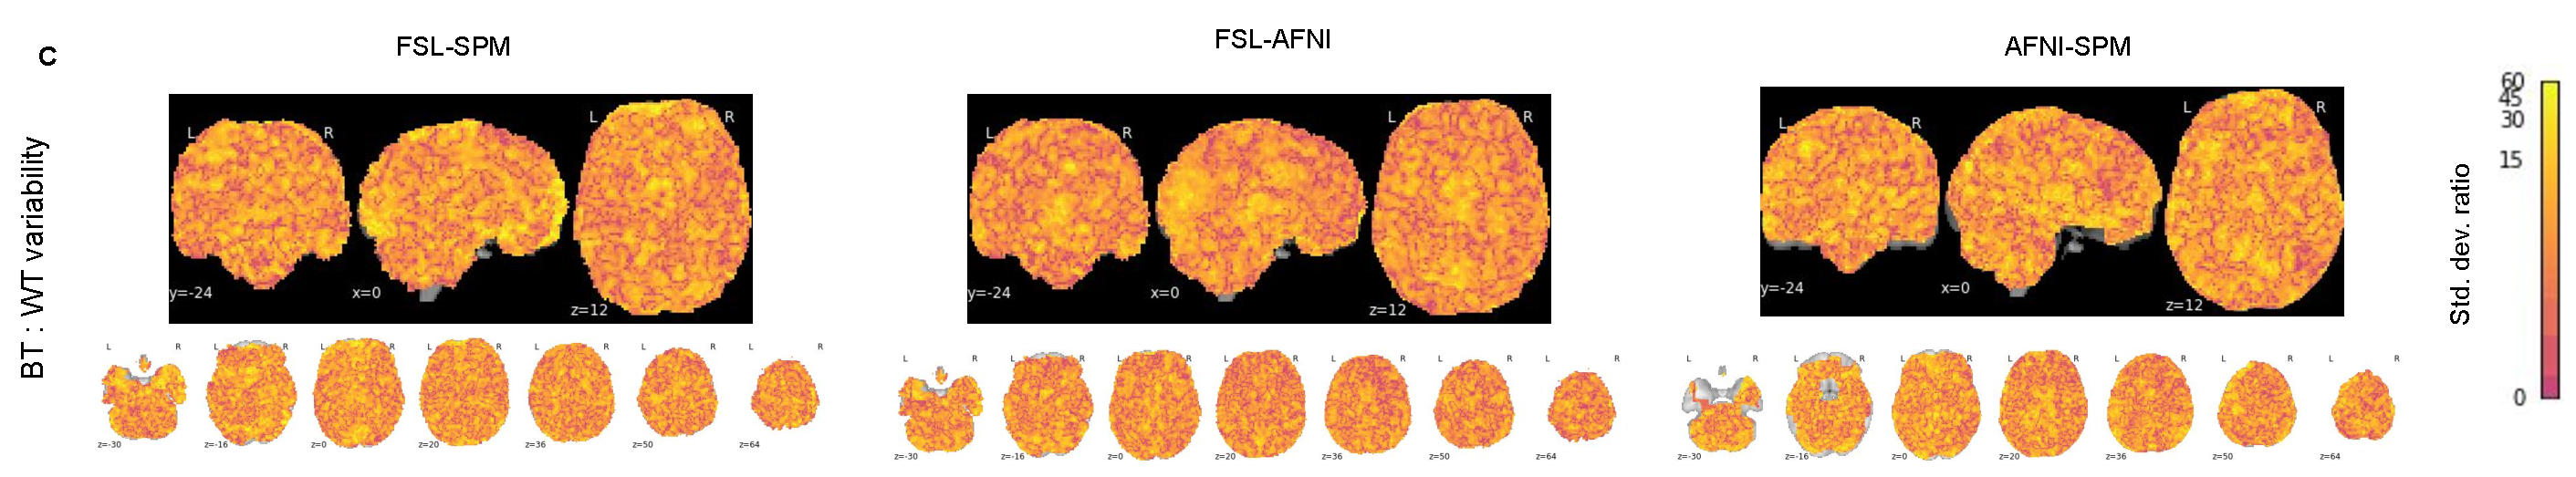
\includegraphics[width=\linewidth]{figures/plots/ratio-unthresh-std.pdf}
    %\caption{Standard deviation of thresholded t-statistics map on template surface}
    \label{fig:unthresh-ratiomaps}
  \end{subfigure}
  \caption{Maps of standard deviation of unthresholded T-statistics. First and second rows show
  maps on between-tool and within-tool results, respectively. Third row represents the ratio of differences
  in between and within tools.}
  \label{fig:unthresh-varmaps}
  \end{minipage}}
\end{figure}


%%%%%%%%%% Corr. plot of tstats%%%%%%%%
\begin{figure}[b]
  \fbox{\begin{minipage}{\dimexpr \textwidth-2\fboxsep-2\fboxrule}
    \begin{subfigure}[t]{\linewidth}
      \centering
      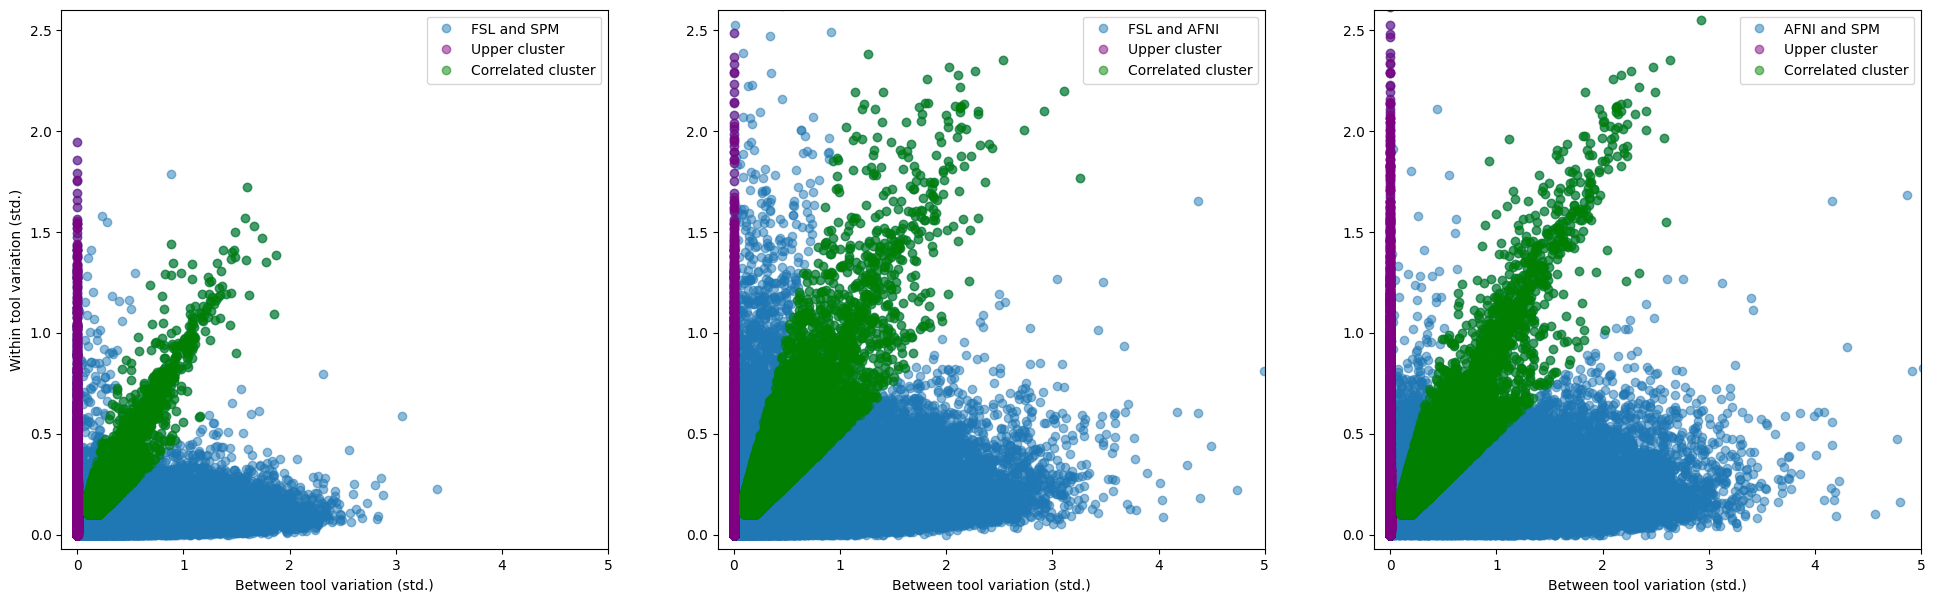
\includegraphics[width=\linewidth]{figures/std-corr-unthresh-plot.png}
      %\caption{Standard deviation of thresholded t-statistics map on template surface}
      \label{fig:unthresh-corrplot}
    \end{subfigure}
    \hfill
    \begin{subfigure}[t]{\linewidth}
      \centering
      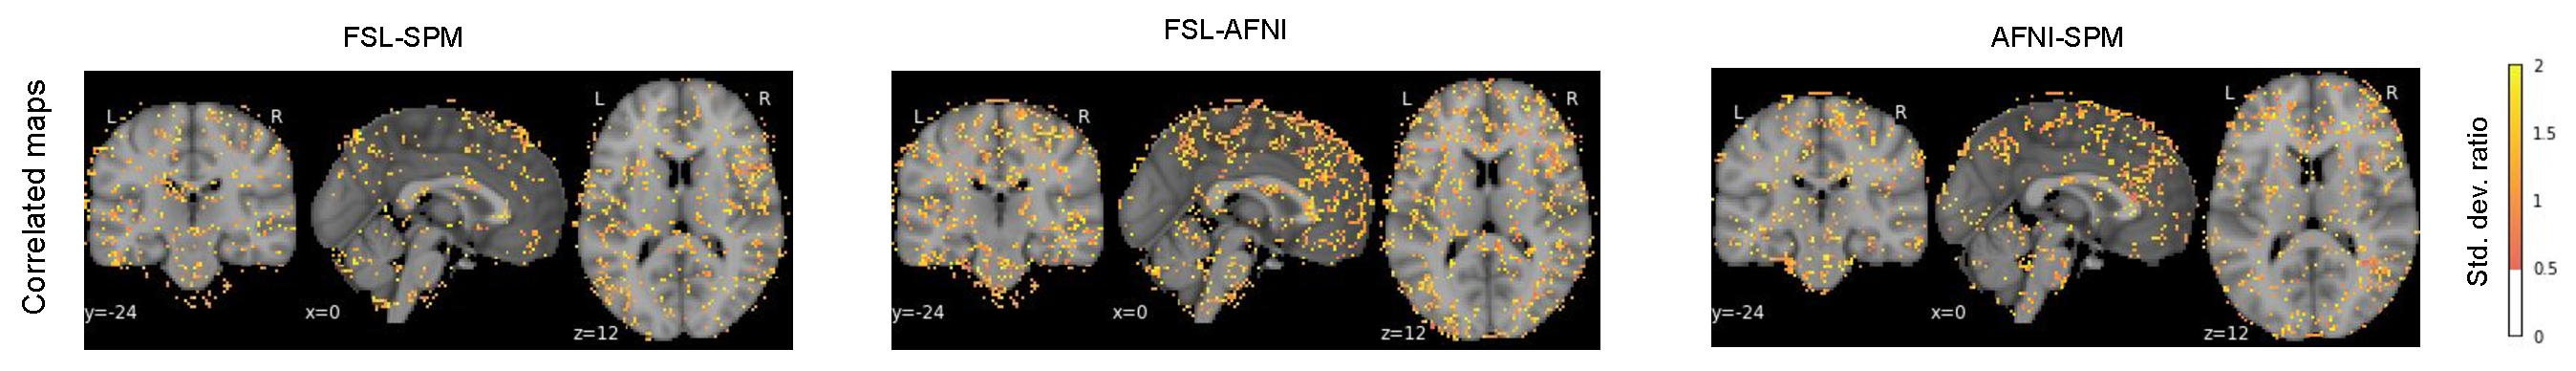
\includegraphics[width=\linewidth]{figures/plots/corr-unthresh-std.pdf}
      %\caption{Standard deviation of thresholded t-statistics map on template surface}
      \label{fig:unthresh-corrmaps}
    \end{subfigure}
    \caption{Correlation of variability in between-tool and within-tool variations in unthresholded maps. First row plots the correlations
  voxel by voxel, which is highlighted with different colors for two major clusters including upper cluster (purple color) and
  correlated cluster (green color) which are mapped on the brain in the second row.}
  \label{fig:correlations}
  \end{minipage}}
\end{figure}


% \subsection{The precision that Fuzzy FSL tool can simulate the between tool variations}
% \begin{description}
%   \item[$\bullet$ Figure 5:] Repeat Fig 1-4 for the results of Fuzzy FSL on the precision that simulate mostly betwen tool varions.
% \end{description}

\section{Conclusion \& Discussion}
% In this study, we represented the magnitude of differences in between tool and within tool results.
% Also we showed the numerically dependent parts of the brain, and explained how between tool variations
% are correlated with numerical variability. Moreover, we indicated the spatial similarity between results so that
% numerical perturbations preserve the topology of the avtivation patterns across all three sets of packages in both conditions.

% Further studies can be evaluating the numerical stabilities within tool by focusing on the particular parts of 
% the pipeline that has been identified as the mian sources of variations in~\cite{bowring2019exploring}. 


%
% ---- Bibliography ----
%
% BibTeX users should specify bibliography style 'splncs04'.
% References will then be sorted and formatted in the correct style.
%
\bibliographystyle{splncs04}
\bibliography{biblio}

\end{document}
